\documentclass{classrep}
\usepackage[utf8]{inputenc}
\usepackage{color}
\usepackage[polish]{babel}
\usepackage[T1]{fontenc}
\usepackage{enumerate}
\usepackage{graphicx}
\usepackage{float}
\restylefloat{table}
\usepackage{multirow}
\usepackage[normalem]{ulem}
\useunder{\uline}{\ul}{}
\selectlanguage{polish}

\studycycle{Informatyka, studia dzienne, I st.}
\coursesemester{VI}

\coursename{Komputerowe systemy rozpoznawania}
\courseyear{2018/2019}

\courseteacher{dr hab. inż. Adam Niewiadomski}
\coursegroup{poniedziałek, 12:15}

\author{
  \studentinfo{Stanisław Zakrzewski}{210360} \and
  \studentinfo{ Maciej Socha}{210321}
}

\title{Zadanie 1: Ekstrakcja cech, miary podobieństwa, klasyfikacja}

\begin{document}
\maketitle
\newpage

\section{Cel}
Celem zadania było poznanie oraz zaimplementowanie różnych metod ekstrakcji cech z tekstów, określania podobieństwa oraz klasyfikacji tekstów.

\section{Wprowadzenie}
	Celem projektu jest stworzenie programu pozwalającego na klasyfikację  wybranego zbioru elementów. Klasyfikatorem wybranym do tego celu jest metoda k-najbliższych sąsiadów.
	
	Algorytm k najbliższych sąsiadów, nazywamy też potocznie algorytmem knn, pozwala na klasyfikację zbioru wieloelementowego według określonych etykiet. Na początku działania algorytmu k najbliższych sąsiadów określane są wektory dla każdego z elementów podlegających klasyfikacji. W naszym przypadku określanie wektorów polega na odpowiednim przetworzeniu tekstu zawierającego się w elementach zbioru do klasyfikacji. Następnie wektory są umieszczane na przestrzeni n elementowej, gdzie n stanowi liczebność elementów w wektorze. Odsłaniane są etykiety, domyślnie 10\% dla każdej z etykiet. Odsłonięcie etykiet stanowi jeden ze sposobów rozwiązania problemu zimnego startu. Następnie kolejne etykiety są nadawane kolejnym elementom, poprzez znalezienie k najbliższych elementów i wybranie spośród etykiet należących do danych elementów tych, które są najliczniejsze, w przypadku identycznej liczebności etykiet wybierana jest ta, której średnia odległość do aktualnie klasyfikowanego elementu jest mniejsza.
	
	Do wytworzenia wektora cech stosowane są dwa warianty ekstrakcji cech typu Dictionary Matching (DM). W obu przypadkach teksty znajdujące się w artykułach są początkowo poddane procesowi lemmatyzacji. Proces lemmatyzacji jest to czynność mająca na celu znalezienia lemmy dla danego słowa, lemma jest to forma podstawowa wyrazu w obszarze części mowy, którą reprezentuje. Następnie następuje proces przyznawania punktów dla poszczególnych słów. Wybierane zostają słowa mające najwięcej punktów. Pierwszy z na początku usuwa wszystkie słowa znajdujące się na przygotowanej wcześniej stop-liście, usuwa wartości liczbowe oraz zwiększa punktację słów znajdujących się bliżej początku tekstu. Drugi sposób bazuje natomiast na algorytmie TFIDF oraz również usuwane są wszelkie wartości liczbowe. 
	
	Algorytm TFIDF jest jedną z metod obliczania wagi słów w oparciu o liczbę ich wystąpień. Jest on stosowany między innymi w wyszukiwarkach internetorych. Jest on obliczany przy pomocy wzoru:
\[ \left ( tf-idf \right )_{i,j}=tf_{i,j} \times idf_{i} \]
gdzie \( tf_{i,j} \) to tak zwany „term frequency” opisany wzorem:
\[ tf_{i,j}=log \frac{n_{i,j}}{\sum _{k}n_{k,j}} \]
gdzie: \( n_{i,j} \) jest liczbą wystąpień termu \( \left ( t_{i} \right ) \) w dokumencie \( d_{j}\), a mianownik jest dumą liczby wystąpień wszystkich termów w dokumencie \( d_{j} \cdot idf_{i} \) to „inverse document frequency” wyraża się wzorem:
\[ idf_{i}=log \frac{|D|}{| \left \{ d: t_{i} \epsilon d \right \} |} \]
gdzie:
\( |D| \) - liczba dokumentów w korpusie
\( | \left \{ d: t_{i} \epsilon d \right \} | \) - liczba dokumentów zawierających przynajmniej jedno wystąpienie danego termu.

	Powstałe w wyniku działania obu ekstraktorów cech wektory są używane do wytworzenia wektorów liczbowych pozwalających na umieszczenie elementów w przestrzeni liczbowej, co jest wymagane w algorytmie k najbliższych sąsiadów.
	
	Obliczenia odległości dokonano w trzech metrykach.
	
	Pierwszą z nich jest metryka Euklidesa, odległość \( d \) obliczana jest przy pomocy wzoru: 
\[ d\left ( x,y \right )=\sqrt{\left ( x_{1}-y_{1} \right )^{2} + \left ( x_{2}-y_{2} \right )^{2} + ... + \left ( x_{n}-y_{n} \right )^{2}} \]

	Drugą z nich jest metryka Manhattana, nazywana również metryką uliczną, taksówkarską lub miejską. Odległość jest obliczana przy pomocy wzoru:
\[ d\left ( x,y \right )=\sum|x_{i}-y_{i}| \]

	Trzecią i zarazem ostatnią jest metryka Czebyszewa, odległość jest obliczana przy pomocy wzoru:
\[ d\left ( x,y \right )=\frac{\sum|x_{i} \cdot y_{i}|}{\sqrt{ \sum x_{i}^{2} \cdot \sum y_{i}^{2} }} \]

	Podobieństwo pomiędzy poszczególnymi słowami wyznaczaliśmy przy pomocy dwóch spobów:
Pierwszym z nich była uogólniona miara n-gramów. Obliczana jest przy pomocy wzoru:

$$ \mu_{N}(s_{1}, s_{2})= \frac{2}{N^{2} + N}  \sum_{i=1}^{N(s_{1})} \sum_{j=1}^{N(s_{1})-i+1}  h(i,j) $$

Drugim były natomiast trigramy. Ich użycie miało na celu pokazanie przewagi uogólnionej miary n-gramów nad miarą z jednym jasno określonym n. Obliczaja jest przy pomocy wzoru:

$$ sim_{n}(s_{1}, s_{2}) = \frac{1}{N - n + 1} \sum_{i = 1}^{N-n+1} h(i) $$

\section{Opis implementacji}
Algorytmy zostały zaimplementowane w języku Java w wersji 11. Dodatkowo na potrzemy procesu lemmatyzacji wykorzystano, udostępnioną przez Stanford Natural Language Processing Group, biliotekę CoreNLP w wersji 3.9.2. Biblioteka ta jest udostępniona z licencją GNU General Public License v3 co pozwala nam korzystać z niej w naszym programie. Biblioteka ta jest bardzo obszerna, w naszym programie wykorzystujemy jedynie funkcjonalność lemmatyzacji. Jest ona zaimplementowana w klasie StanfordLemmatizer. Implementacja tej klasy została bezpośrednio zaczerpnięta z dokumentacji[5]. Poniżej przedstawiono uproszczony diagram klas. Zaznaczone zostały na nim kluczowe dla działania naszego programu klasy.\\

\begin{figure}[ht]
	\makebox[\linewidth]{
		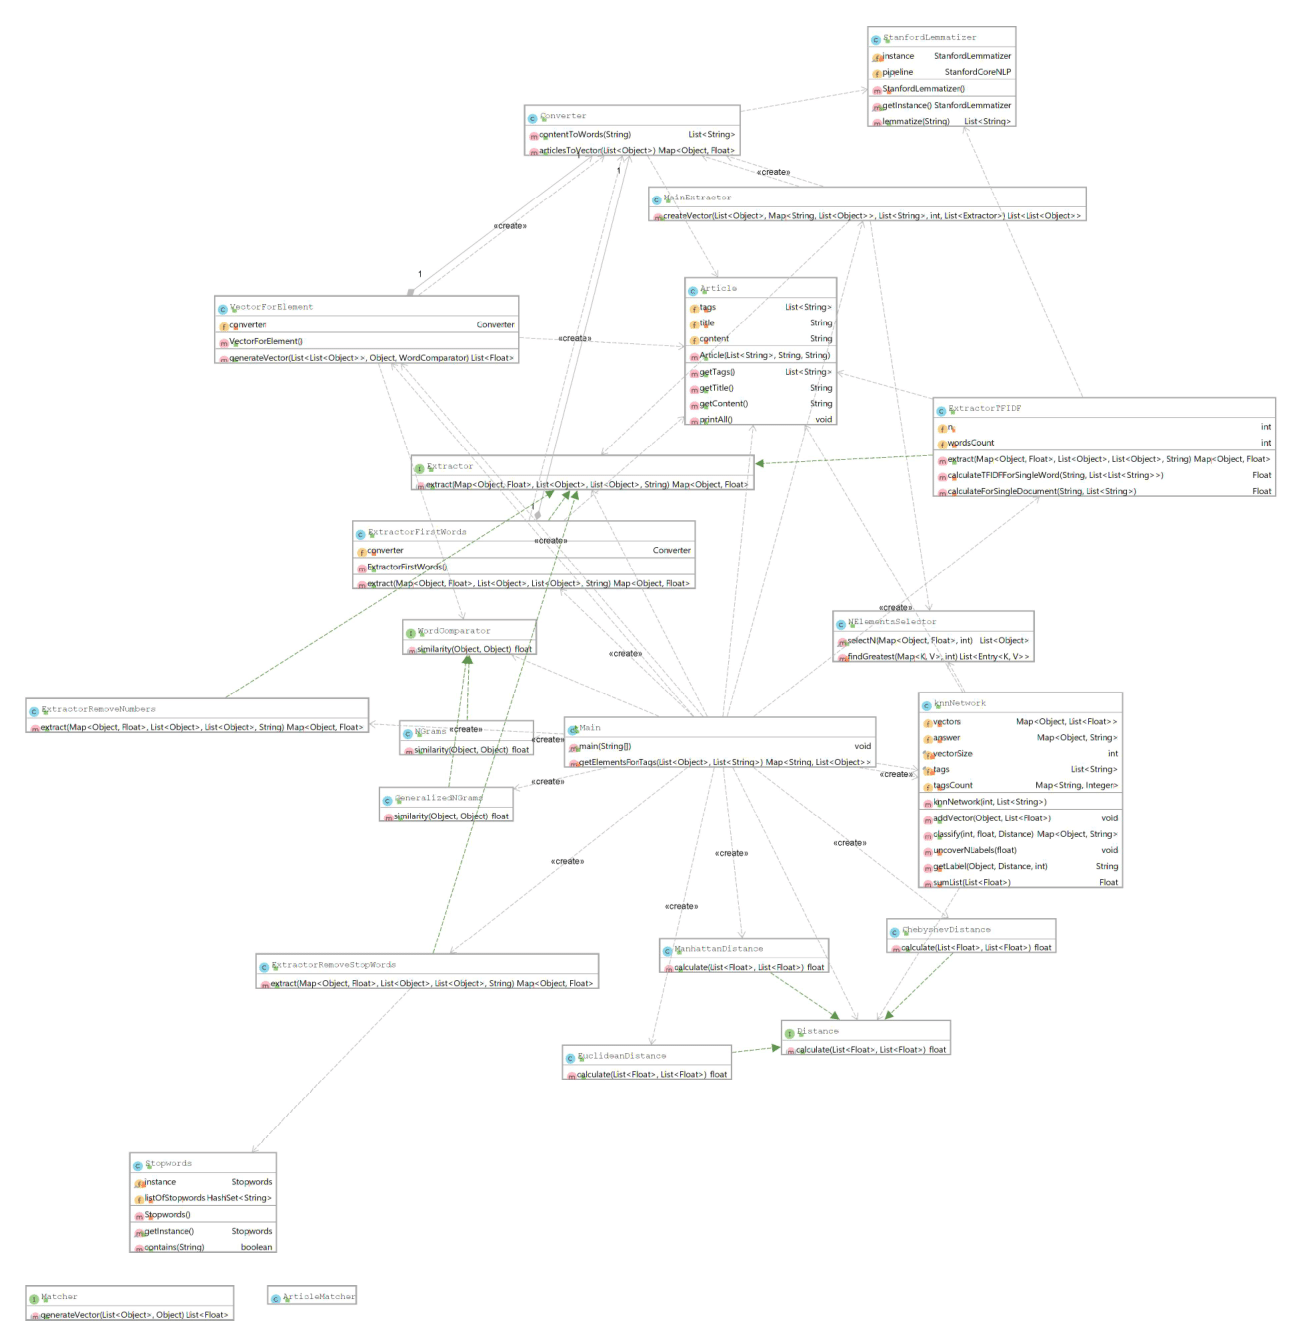
\includegraphics[scale=0.4]{uml.png}
	}
	\caption{UML Diagram}
\end{figure}

Klasa Article odpowiada za przechowywanie informacji niezbędnych do działania programu. Wykorzystujemy ją zarówno do przetwarzania artukułów zawartych w zbiorze danych reuters jak i zestawu artykułów przygotowanego przez nas samych.\\
Interfejs Extractor służy i znajdująca się w nim metoda extract jest wykorzystywana przy procesie ekstakcji cech. Implementują ją liczne klasy zawierające sie w dwóch sposobach ekstarakcji cech zawartych w programie.\\
Klasa knnNetwork zawiera w sobie implementację algorytmu k najbliższych sąsiadów do ustalania przynależności wektorów odpowiadającycm przekazanym do programu elementom. Klasa pozwala na dodawanie wektorów wraz z odpowiadającymi im elementami, a następnie klasyfikowanie ich przy przekazaniu odpowiedniego parametru k oznaczającego liczbę sąsiadów, uncoveredLabelFraction zapomocą którego przekazujemy jaka część tekstów będzie miała odkryte etykiety oraz distance, metrykę obliczania dystansu pomiędzy wektorami.\\
Pakiet calculatedistance zawiera w sobie interfejs Distance oraz implementujące go klasy ChebyshevDistance(metryka Czebyszewa), EuclideanDistance(metryka Euklidesa) oraz ManhattanDistance(metryka uliczna). Są to wymagane przez treść zadania metryki pomiaru odległości pomiędzy wektorami.\\
Za przekazywanie danych do programu odpowiada plik config.txt zawierający w sobie wszystkie potrzebne do działania programu parametry. Są to odpowiednio:
\begin{itemize}
	\item tagClass - tag dla którego etykiety będzie nadawał program
	\item folderPath - ścieżka do folderu z plikami z danymi
	\item articlesToReadCount - liczba plików z artykułami, które program ma wczytać
	\item k - liczba najbliższych sąsiadów według których algorytm będzie klasyfikował
	\item fractionOfUncoveredForEachTag - część elementów należących do każdej z etykiet, która ma zostać odkryta w klasyfikacji knn
	\item tags - etykiety, według których program ma klasyfikować
	\item numberOfElementsPerTag - liczba elementów jakie ma zawierać w sobie cecha dla każdej z etykiet
	\item trainToTestRatio - stosunek zbioru treningowego do testowego
	\item distanceKNN - metryka pomiaru dystansu w przestrzeni dla algorytmu knn
	\item wordSimilarity - metryka podobieństwa słów
	\item extractors - zestaw ekstraktorów
\end{itemize}


\section{Materiały i metody}
Klasyfikacja tekstów Reutersa oraz danych zebranych przez nas została wykonana dla obu sposobów ekstrakcji cech i dla każdej z 3 metryk obliczania dystansu w algorytmie k najbliższych sąsiadów. Dla parametru k wybrano niektóre wartości ze zbioru (3, 5, 8, 11, 19), tak aby jak najlepiej ukazać właściwości każdego z sposobów ekstrakcji oraz najlepiej dopasować je do zbioru danych testowych. Klasyfikacja na zbiorze Reutersa według tagu PLACES została przeprowadzona dla sześciu etykiet (west-germany, usa, uk, canada, france, japan), przy stosunku zbioru treningowego do testowego 60-40 i dla 10\% odkrytych etykiet. W drugim przypadku według tagu TOPICS etykietowano przy pomocy dwóch etykiet (coffee i gold), przy równym podziale na zbiór treningowy i testowy. Natomiast w naszych tekstach klasyfikacja nastąpiła według tagu REVIEWS dla dwóch etykiet (movie, restaurant), równego podziału zbioru elementów na część treningową i testową oraz 20\% odkrytych etykiet.

\section{Wyniki}
Wyniki kolejnych przeprowadzanych eksperymentów zostały umieszczone w tabelach poniżej. Początkowa konfiguracja programu znajduje się poniżej, przy kolejnych eksperymentach zostały wspominanie tylko te parametry które były zmienione.
\begin{itemize}
	\item tagClass = PLACES
	\item articlesToReadCount = 23
	\item k = 3
	\item fractionOfUncoveredForEachTag = 0.1
	\item tags = west-germany, usa, france, uk, canada, japan
	\item numberOfElementsPerTag = 5
	\item trainToTestRatio = 0.6
	\item distanceKNN = euclidean
	\item wordSimilarity = NGrams
	\item extractors = 1
\end{itemize}
Poniżej znajdują się wyniki dla przedstawionych powyższej parametrów.\\


\begin{table}[H]
\begin{tabular}{|c|c|c|}
\hline
Label        & Precision  & Recall     \\ \hline
west-germany & 0.39534885 & 0.3923077  \\ \hline
usa          & 0.83159405 & 0.9416126  \\ \hline
france       & 0.5064935  & 0.35779816 \\ \hline
uk           & 0.62025315 & 0.24873096 \\ \hline
canada       & 0.49079755 & 0.23738873 \\ \hline
japan        & 0.5652174  & 0.23636363 \\ \hline
\end{tabular}
\caption{Precision i Recall dla parametrów bazowych}
\end{table}
Multi-Class Pecision: 0.7962223\\
\\
\\
\begin{table}[H]
\begin{tabular}{|c|c|c|c|c|c|c|}
\hline
             & west-germany & usa  & france & uk & canada & japan \\ \hline
west-germany & 51           & 74   & 0      & 2  & 3      & 0     \\ \hline
usa          & 57           & 4064 & 31     & 57 & 71     & 36    \\ \hline
france       & 1            & 65   & 39     & 0  & 2      & 2     \\ \hline
uk           & 10           & 273  & 5      & 98 & 7      & 1     \\ \hline
canada       & 5            & 248  & 2      & 1  & 80     & 1     \\ \hline
japan        & 5            & 163  & 0      & 0  & 0      & 52    \\ \hline
\end{tabular}
\caption{Przypisanie tagów dla parametrów bazowych}
\end{table}
\newpage

\subsection{Eksperymenty 1 - Różne metryki odległości}
Metryka euklidesowa
\begin{table}[H]
\begin{tabular}{|c|c|c|}
\hline
Label        & Precision  & Recall     \\ \hline
west-germany & 0.39534885 & 0.3923077  \\ \hline
usa          & 0.83159405 & 0.9416126  \\ \hline
france       & 0.5064935  & 0.35779816 \\ \hline
uk           & 0.62025315 & 0.24873096 \\ \hline
canada       & 0.49079755 & 0.23738873 \\ \hline
japan        & 0.5652174  & 0.23636363 \\ \hline
\end{tabular}
\caption{Precision i Recall dla metryki euklidesowej}
\end{table}
Multi-Class Pecision: 0.7962223\\
\\
\\
Metryka uliczna
\begin{table}[H]
\begin{tabular}{|c|c|c|}
\hline
Label        & Precision  & Recall     \\ \hline
west-germany & 0.5566038  & 0.4402985  \\ \hline
usa          & 0.8411453  & 0.914457   \\ \hline
france       & 0.32407406 & 0.2651515  \\ \hline
uk           & 0.45026177 & 0.22994652 \\ \hline
canada       & 0.45614034 & 0.31610942 \\ \hline
japan        & 0.53797466 & 0.425      \\ \hline
\end{tabular}
\caption{Precision i Recall dla metryki ulicznej}
\end{table}
Multi-Class Pecision: 0.78732294\\
\\
\\
Metryka Czebyszewa
\begin{table}[H]
\begin{tabular}{|c|c|c|}
\hline
Label        & Precision  & Recall     \\ \hline
west-germany & 0.64788735 & 0.35384616 \\ \hline
usa          & 0.8515893  & 0.91464823 \\ \hline
france       & 0.37195122 & 0.5126051  \\ \hline
uk           & 0.4652778  & 0.17539267 \\ \hline
canada       & 0.52517986 & 0.43843845 \\ \hline
japan        & 0.49222797 & 0.4589372  \\ \hline
\end{tabular}
\caption{Precision i Recall dla metryki Czebyszewa}
\end{table}
Multi-Class Pecision: 0.7954958
\newpage

\subsection{Eksperymenty 2 - różne metryki porównywania słów}
NGramy dla n = 3
\begin{table}[H]
\begin{tabular}{|c|c|c|}
\hline
Label        & Precision  & Recall     \\ \hline
west-germany & 0.39534885 & 0.3923077  \\ \hline
usa          & 0.83159405 & 0.9416126  \\ \hline
france       & 0.5064935  & 0.35779816 \\ \hline
uk           & 0.62025315 & 0.24873096 \\ \hline
canada       & 0.49079755 & 0.23738873 \\ \hline
japan        & 0.5652174  & 0.23636363 \\ \hline
\end{tabular}
\caption{Precision i Recall dla NGramów, n = 3}
\end{table}
Multi-Class Pecision: 0.7962223\\
\\
\\
NGramy dla n = 2
\begin{table}[H]
\begin{tabular}{|c|c|c|}
\hline
Label        & Precision  & Recall     \\ \hline
west-germany & 0.5416667  & 0.104      \\ \hline
usa          & 0.80586374 & 0.94232106 \\ \hline
france       & 0.22972973 & 0.16037735 \\ \hline
uk           & 0.26666668 & 0.12276215 \\ \hline
canada       & 0.4347826  & 0.16574585 \\ \hline
japan        & 0.47619048 & 0.09756097 \\ \hline
\end{tabular}
\caption{Precision i Recall dla NGramów, n = 2}
\end{table}
Multi-Class Pecision: 0.7675263\\
\\
\\
NGramy dla n = 4
\begin{table}[H]
\begin{tabular}{|c|c|c|}
\hline
Label        & Precision  & Recall     \\ \hline
west-germany & 0.5652174  & 0.36879432 \\ \hline
usa          & 0.847703   & 0.9302486  \\ \hline
france       & 0.36619717 & 0.23853211 \\ \hline
uk           & 0.41411042 & 0.34526855 \\ \hline
canada       & 0.6785714  & 0.23312883 \\ \hline
japan        & 0.6884058  & 0.4871795  \\ \hline
\end{tabular}
\caption{Precision i Recall dla NGramów, n = 4}
\end{table}
Multi-Class Pecision: 0.80366874\\
\\
\\
\\
\\
\\
Uogólnione NGramy
\begin{table}[H]
\begin{tabular}{|c|c|c|}
\hline
Label        & Precision  & Recall      \\ \hline
west-germany & 0.7589286  & 0.65891474  \\ \hline
usa          & 0.8819797  & 0.9648311   \\ \hline
france       & 0.46666667 & 0.7241379   \\ \hline
uk           & 0.7490196  & 0.49354005  \\ \hline
canada       & 1.0        & 0.099415205 \\ \hline
japan        & 0.76649743 & 0.7190476   \\ \hline
\end{tabular}
\caption{Precision i Recall dla UogólnionychNGramów}
\end{table}
Multi-Class Pecision: 0.85633856

\subsection{Eksperymenty 3 - Różne wartości parametru k}
k = 3
\begin{table}[H]
\begin{tabular}{|c|c|c|}
\hline
Label        & Precision  & Recall     \\ \hline
west-germany & 0.39534885 & 0.3923077  \\ \hline
usa          & 0.83159405 & 0.9416126  \\ \hline
france       & 0.5064935  & 0.35779816 \\ \hline
uk           & 0.62025315 & 0.24873096 \\ \hline
canada       & 0.49079755 & 0.23738873 \\ \hline
japan        & 0.5652174  & 0.23636363 \\ \hline
\end{tabular}
\caption{Precision i Recall dla k = 3}
\end{table}
Multi-Class Pecision: 0.7962223\\
\\
\\
k = 5
\begin{table}[H]
\begin{tabular}{|c|c|c|}
\hline
Label        & Precision  & Recall     \\ \hline
west-germany & 0.59       & 0.43382353 \\ \hline
usa          & 0.83722854 & 0.93855786 \\ \hline
france       & 0.46666667 & 0.26168224 \\ \hline
uk           & 0.46025103 & 0.28795812 \\ \hline
canada       & 0.6566265  & 0.29945055 \\ \hline
japan        & 0.5660377  & 0.29411766 \\ \hline
\end{tabular}
\caption{Precision i Recall dla k = 5}
\end{table}
Multi-Class Pecision: 0.8016709\\
\\
\\
\\
\\
\\
\\
k = 8
\begin{table}[H]
\begin{tabular}{|c|c|c|}
\hline
Label        & Precision  & Recall     \\ \hline
west-germany & 1.0        & 0.09375    \\ \hline
usa          & 0.8347242  & 0.95040554 \\ \hline
france       & 0.44827586 & 0.10655738 \\ \hline
uk           & 0.6        & 0.29210526 \\ \hline
canada       & 0.625      & 0.375      \\ \hline
japan        & 0.58278143 & 0.43781096 \\ \hline
\end{tabular}
\caption{Precision i Recall dla k = 8}
\end{table}
Multi-Class Pecision: 0.81002545\\
\\
\\
k = 13
\begin{table}[H]
\begin{tabular}{|c|c|c|}
\hline
Label        & Precision  & Recall      \\ \hline
west-germany & 0.61290324 & 0.2753623   \\ \hline
usa          & 0.8147582  & 0.98611754  \\ \hline
france       & 1.0        & 0.094339624 \\ \hline
uk           & 1.0        & 0.09793814  \\ \hline
canada       & 0.67832166 & 0.297546    \\ \hline
japan        & 1.0        & 1.0         \\ \hline
\end{tabular}
\caption{Precision i Recall dla k = 13}
\end{table}
Multi-Class Pecision: 0.81129676\\
\\
\\
k = 21
\begin{table}[H]
\begin{tabular}{|c|c|c|}
\hline
Label        & Precision  & Recall     \\ \hline
west-germany & 1.0        & 0.09375    \\ \hline
usa          & 0.81465435 & 0.9944815  \\ \hline
france       & 1.0        & 0.09615385 \\ \hline
uk           & 1.0        & 0.104      \\ \hline
canada       & 0.7826087  & 0.26548672 \\ \hline
japan        & 1.0        & 0.09952607 \\ \hline
\end{tabular}
\caption{Precision i Recall dla k = 21}
\end{table}
Multi-Class Pecision: 0.81674534
\newpage

\subsection{Eksperymenty 4 - Różne ekstraktory}
Ekstraktor nr 1
\begin{table}[H]
\begin{tabular}{|c|c|c|}
\hline
Label        & Precision  & Recall     \\ \hline
west-germany & 0.39534885 & 0.3923077  \\ \hline
usa          & 0.83159405 & 0.9416126  \\ \hline
france       & 0.5064935  & 0.35779816 \\ \hline
uk           & 0.62025315 & 0.24873096 \\ \hline
canada       & 0.49079755 & 0.23738873 \\ \hline
japan        & 0.5652174  & 0.23636363 \\ \hline
\end{tabular}
\caption{Precision i Recall dla ekstraktora 1.}
\end{table}
Multi-Class Pecision: 0.7962223\\
\\
Ekstraktor nr 2
articlesToReadCount = 10
\begin{table}[H]
\begin{tabular}{|c|c|c|}
\hline
Label        & Precision  & Recall      \\ \hline
west-germany & 0.17948718 & 0.13461539  \\ \hline
usa          & 0.81395346 & 0.94287044  \\ \hline
france       & 0.6363636  & 0.1         \\ \hline
uk           & 0.30555555 & 0.17837837  \\ \hline
canada       & 0.6060606  & 0.104166664 \\ \hline
japan        & 0.19444445 & 0.10144927  \\ \hline
\end{tabular}
\caption{Precision i Recall dla ekstraktora 2.}
\end{table}
Multi-Class Pecision: 0.77324516

\subsection{Eksperymenty 5 - Inny tag}
Eksperymenty dla tagu TOPICS oraz etykiet coffe, gold.
\begin{table}[H]
\begin{tabular}{|c|c|c|}
\hline
Label  & Precision & Recall    \\ \hline
coffee & 0.9811321 & 0.9122807 \\ \hline
gold   & 0.9074074 & 0.98      \\ \hline
\end{tabular}
\caption{Precision i Recall dla tagu TOPISC}
\end{table}
Multi-Class Pecision: 0.94392526\\
\\
\\
distance = manhattan
\begin{table}[H]
\begin{tabular}{|c|c|c|}
\hline
Label  & Precision  & Recall     \\ \hline
coffee & 0.94827586 & 0.94827586 \\ \hline
gold   & 0.93877554 & 0.93877554 \\ \hline
\end{tabular}
\caption{Precision i Recall dla tagu TOPISC i dystansu miejskiego}
\end{table}
Multi-Class Pecision: 0.94392526\\
\\
\\
distance = chebyshev
\begin{table}[H]
\begin{tabular}{|c|c|c|}
\hline
Label  & Precision  & Recall     \\ \hline
coffee & 0.98245615 & 0.9655172  \\ \hline
gold   & 0.96       & 0.97959185 \\ \hline
\end{tabular}
\caption{Precision i Recall dla tagu TOPISC i dystansu Czebyszewa}
\end{table}
Multi-Class Pecision: 0.97196263\\
\\
extractors = 2
\begin{table}[H]
\begin{tabular}{|c|c|c|}
\hline
Label  & Precision & Recall      \\ \hline
coffee & 0.6213592 & 1.0         \\ \hline
gold   & 1.0       & 0.093023255 \\ \hline
\end{tabular}
\caption{Precision i Recall dla tagu TOPISC i 2. ekstraktora}
\end{table}
Multi-Class Pecision: 0.635514\\
\\
trainToTestRatio = 0.3
\begin{table}[H]
\begin{tabular}{|c|c|c|}
\hline
Label  & Precision & Recall    \\ \hline
coffee & 0.975     & 0.975     \\ \hline
gold   & 0.9714286 & 0.9714286 \\ \hline
\end{tabular}
\caption{Precision i Recall dla tagu TOPISC i stosunku zbiorów 0.3}
\end{table}
Multi-Class Pecision: 0.97333336\\
\\
k = 5
\begin{table}[H]
\begin{tabular}{|c|c|c|}
\hline
Label  & Precision  & Recall \\ \hline
coffee & 0.91935486 & 1.0    \\ \hline
gold   & 1.0        & 0.9    \\ \hline
\end{tabular}
\caption{Precision i Recall dla tagu TOPISC i k = 5}
\end{table}
Multi-Class Pecision: 0.95327103

\subsection{Eksperymenty 6 - Nasz zbiór tekstów}
\begin{table}[H]
\begin{tabular}{|c|c|c|}
\hline
Label      & Precision & Recall      \\ \hline
movie      & 0.5641026 & 1.0         \\ \hline
restaurant & 1.0       & 0.055555556 \\ \hline
\end{tabular}
\caption{Precision i Recall dla własnych tekstów}
\end{table}
Multi-Class Pecision: 0.575\\
\\
\\
Uogólniona miara Ngramów
\begin{table}[H]
\begin{tabular}{|c|c|c|}
\hline
Label      & Precision  & Recall     \\ \hline
movie      & 0.72727275 & 0.8888889  \\ \hline
restaurant & 0.8888889  & 0.72727275 \\ \hline
\end{tabular}
\caption{Precision i Recall dla własnych tekstów i uogólnionej miary NGramów}
\end{table}
Multi-Class Pecision: 0.8\\
\\
\\
k = 8
\begin{table}[H]
\begin{tabular}{|c|c|c|}
\hline
Label      & Precision & Recall     \\ \hline
movie      & 0.5897436 & 1.0        \\ \hline
restaurant & 1.0       & 0.05882353 \\ \hline
\end{tabular}
\caption{Precision i Recall dla własnych tekstów i uogólnionej miary NGramów}
\end{table}
Multi-Class Pecision: 0.6

\section{Dyskusja}
	Napisanie programu klasyfikującego uświadomiło nam, że w rozpoznawaniu danego tekstu nie liczą się jedynie znaczenia poszczególnych słów. Pozytywny wpływ na jakość klasyfikacji miało między innymi dodanie do ekstrakcji cech „punktowanie” słów znajdujących się bliżej początku artykułu. Właściwość ta jest związana z podstawowymi założeniami artykułu prasowego, i w tekstach opracowanych przez nas recenzji, które mają na celu w pierwszych słowach określić kontekst danego tekstu. Zdajemy sobie sprawę, że dla innego typu tekstu pisanego, takiego jak na przykład opowiadanie cecha ta niekoniecznie będzie obecna, nastąpi wtedy konieczność stworzenia nowego modelu ekstrakcji cech, do którego przyjęcia nasz program jest zdolny.
	
	Zauważyliśmy, że uogólniona miara n-gramów pozwala na osiągnięcie lepszych wyników klasyfikacyjnych od trigramów. Dzieje się tak, ponieważ uogólniona miara n-gramów pozwala na wyższy stopień rozgraniczenia podobieństwa tekstów, poprzez uwzględnienie aspektów niebędących możliwymi do wyłapania w przypadku trigramów. Jedynym przeciwwskazaniem w użyciu uogólnionej miary n-gramów może być jej wyższa złożoność obliczeniowa.
	
	Z trzech miar pomiaru odległości między wektorami, najlepsze rezultaty daje według naszych badań metryka Euklidesa, zaraz za nią jest metryka Czebyszewa, natomiast na końcu plasuje się metryka uliczna. Dystans Euklidesa najlepiej więc oddaje odległość pomiędzy wektorami w przestrzeni dla zastosowania algorytmu k najbliższych sąsiadów.
	
	Algorytm TFIDF okazał się wolniejszy od alternatywnego rozwiązania w drugim sposobie ekstrakcji. Jest to spowodowane jego złożonością obliczeniową w porównaniu do usuwania słów ze stop listy i punktowaniu słów pojawiających się wcześniej. Osiągał on też mniejsze wartości. Jest on jednak w przeciwieństwie do stworzonej przez nas stop-listy uniwersalny.
	
	Normalizacja wektorów cech okazała się niezwykle kluczowa ze względu na różną długość artykułów i recenzji znajdujących się w zbiorach danych. Początkowe próby działania programu bez uniezależnienia wartości na wektorze od długości tekstów dawały bardzo niskie rezultaty.
	
	Rezultaty dla przygotowywanych przez nas tekstów były znacząco niższe niż dla tekstów zaczerpniętych z bazy Reutera. Jest to zapewnie spowodowane spójnym stylem i określoną formą tekstów Reutera, podczas gdy przygotowane przez nas teksty znacząco się różniły pod względem stylistycznym jak i formalnym.
	
	Program osiągnął średnią skuteczność na poziomie 90-95 procent dla tylko dwóch etykiet. Jest to przewidywany efekt. Skuteczność wzrastała nawet do 97 procent po zwiększeniu k z 3 do 5. Jest to wynik więcej niż satysfakcjonujący.

\section{Wnioski}
	Stworzenie systemu ekstrakcji cech dla danego rodzaju bądź zbioru tekstów jest zadaniem o wiele trudniejszym niż przypuszczaliśmy i wymaga nie tylko wiedzy o słowach jakie mogą się znaleźć w danym tekście, ale i dogłębnej wiedzy o wybranym typie tekstu, jak w naszym przypadku artykule jak i w wybranym przez nas, podobnej jeśli chodzi o cechy recenzji.
	
	Algorytm k najbliższych sąsiadów ma problem, w momencie, kiedy jedna z etykiet ma znacząco więcej przyporządkowanych do niej elementów. Ważne jest wtedy aby odpowiednio dobrać wartość k aby nie była zbyt wysoka. Należy też wtedy zadbać o to, aby do zbioru początkowo odkrytych etykiet dla elementów trafiły etykiety każdego rodzaju.
	
	Uniwersalne metody zawsze będą mniej skuteczne niż metody skrojone dokładnie pod dany przypadek. Jest to uniwersalna prawda, która w informatyce odgrywa znaczącą rolę w porównaniu do innych dziedzin. Mogliśmy ją zaobserwować na przykładzie porównania algorytmu TFIDF z stop-listą i wybieraniem słów pojawiających się wcześniej.


\begin{thebibliography}{0}
  \bibitem{article1} David D. Lewis.
  	\textsl{Feature Selection and Feature Extract ion for Text Categorization}, University of Chicago,\\
  	Dostępny w Internecie: \url {https://aclweb.org/anthology/H92-1041?fbclid=IwAR248ftiyFqXrFpi51IDLorT7Ngso369BPTOaOeSYE3QGG1gYD9TNfy58qc}

  \bibitem{article2} David Dolan Lewis.
  	\textsl{Representation and learning in information retrieval}, University of Massachusetts,\\
  	Dostępny w Internecie: \url {http://ciir.cs.umass.edu/pubfiles/UM-CS-1991-093.pdf}

  \bibitem{article3} David D. Lewis.
  	\textsl{Data Extraction as Text Categorization : An
Experiment With the MUC-3 Corpus}, University of Chicago,\\
	Dostępny w Internecie: \url {https://www.aclweb.org/anthology/M91-1035}

  \bibitem{article4} Marina Sokolova, Guy Lapalme.
  	\textsl{A systematic analysis of performance measures for classification tasks}, Information Processing and Management no 45,\\
  	Dostępny w internecie: \url {http://rali.iro.umontreal.ca/rali/sites/default/files/publis/SokolovaLapalme-JIPM09.pdf?fbclid=IwAR2M7_a4QxL_F4yCOB_Akp4ghkoUKrBnHT9xzCfuTcoVrLBe3lN3kIlPt00}

  \bibitem{stanford} Dokumentacja Stanford CoreNLP
    \url {https://stanfordnlp.github.io/CoreNLP}
    
  \bibitem{notatki} Adam Niewiadomski.
  	\textsl{Materiały, przykłady i ćwiczenia do przedmiotu
Komputerowe Systemy Rozpoznawania}, 21 września 2009.\\

\end{thebibliography}
\end{document}
